\begin{figure}[htbp]

\begin{center}
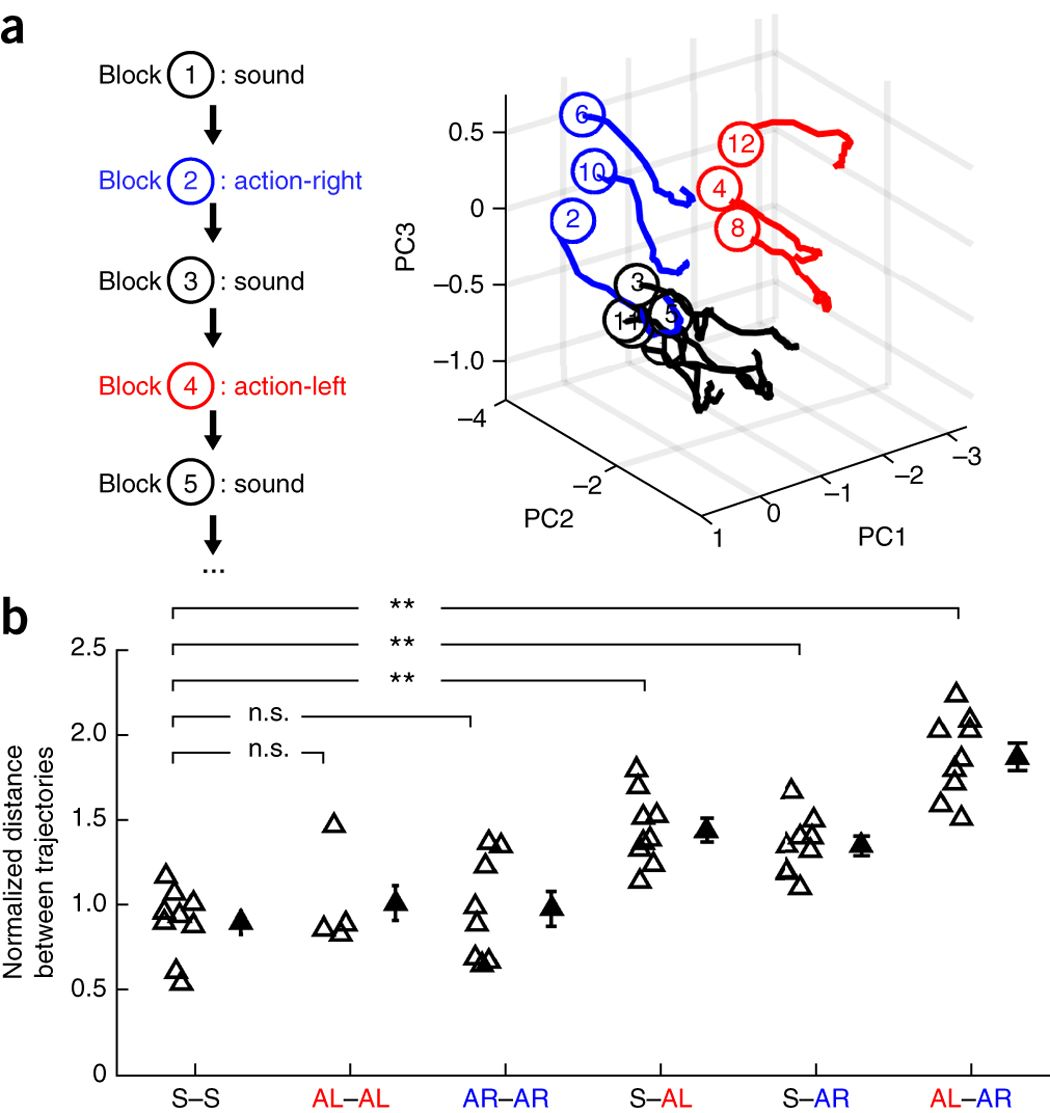
\includegraphics[width=8.7cm]{Figures/Chapter3/NN_fig6} %[width=11.4cm]
\end{center}

\caption[M2 ensembles revisited previous activity patterns upon re-exposure to corresponding rule]
{
M2 ensembles revisited previous activity patterns upon re-exposure to corresponding rule.
(a) Neural circuit trajectories calculated from trial-averaged $\Delta F/F$ for each trial block during one behavioral session. Circled numbers, temporal order in which trial blocks were presented. Open circles, time of response. Black, sound rule. Blue, action-right. Red, action-left. (b) Normalized distance between neural circuit trajectories from different trial types across all experiments (see Methods) for sound (S), action-left (AL) and action-right (AR). Open triangles, median distances from individual experiments. Solid triangles, $\mathit{mean}\pm\mathit{SEM}$. Wilcoxon signed-rank test: S--S vs. AL--AL: $p = 0.6$, $W = 3$; S--S vs. AR--AR: $p = 0.5$, $W = 13$; S--S vs. S--AL: $p = 0.004$, $W = 0$; S--S vs. S--AR: $p = 0.004$, $W = 0$; S--S vs. AL--AR: $p = 0.004$, $W = 0$; **$p < 0.01$. $N = 9$ sessions from 5 mice, except for AL--AL ($N = 4$) and AR--AR ($N = 8$) because mice did not perform enough switches to experience the same block type again in some sessions. **$p < 0.01$; n.s., not significant.
}

\label{fig:NN_fig6}
\end{figure}